	Hacemos una validación cruzada para una muestra de data de 906130 sesiones de usuarios para probar como se comporta con {cross validation}.
	
	
	
	\begin{figure}[h] 
		\centering
			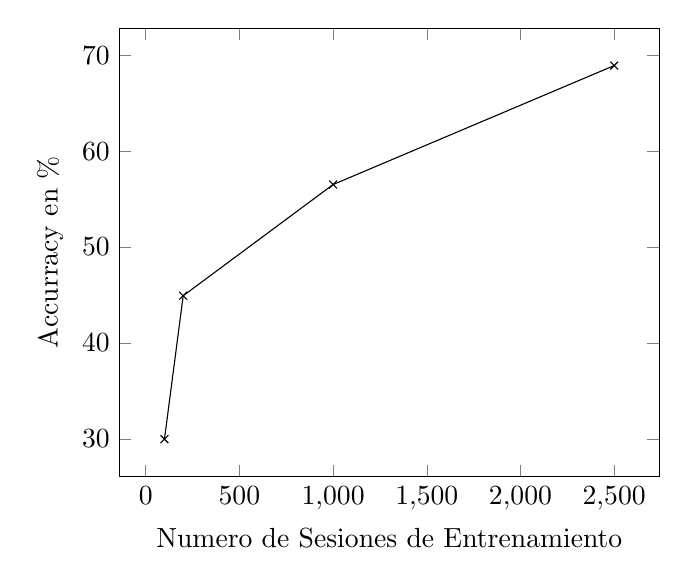
\begin{tikzpicture}
			\begin{axis}[
			xlabel= Numero de Sesiones de Entrenamiento,
			ylabel=Accurracy en \% ]
			\addplot[color=black,mark=x] coordinates {
				(100, 29.9674371114825)
				(200, 44.9237667712101)
				(1000, 56.519572924979)
				(2500, 68.9237667712101)	
			};
			\end{axis}
			\end{tikzpicture}
		\caption{Gráfico de Accuracy vs sesiones de entrenamiento para una cota superior de 5 símbolos}
		\label{fig:sim}
	\end{figure}